\documentclass[12pt]{article}
\usepackage[utf8]{inputenc}
\usepackage{amsmath}
\usepackage{graphicx}
\usepackage{subcaption}
\usepackage{geometry}
\geometry{a4paper, margin=1in}
\usepackage{booktabs}
\usepackage{caption}
\usepackage{listings}
\usepackage{xcolor}

% Configuring listings for Python code
\lstset{
    language=Python,
    basicstyle=\ttfamily\small,
    keywordstyle=\color{blue},
    stringstyle=\color{red},
    commentstyle=\color{green!50!black},
    numbers=left,
    numberstyle=\tiny,
    stepnumber=1,
    numbersep=5pt,
    showspaces=false,
    showstringspaces=false,
    frame=single,
    breaklines=true,
    breakatwhitespace=true,
    tabsize=4
}

% Document setup
\title{Thermocouple Temperature Measurement Simulation Project Report}
\author{}
\date{September 2025}

\begin{document}

\maketitle

\section*{Execution Objective}
The objective of this project is to simulate a temperature measurement system using a Type K thermocouple in a software environment. The simulation includes generating a varying temperature profile, converting it to voltage output based on the thermocouple's sensitivity, adding realistic Gaussian noise to mimic sensor and environmental interference, applying a low-pass Butterworth filter to reduce the noise, and calibrating the filtered voltage back to temperature. The project evaluates the effectiveness of signal processing techniques in instrumentation by comparing the root mean square error (RMSE) before and after filtering. This is an instant, no-hardware project implemented in Python using libraries like NumPy, SciPy, and Matplotlib, runnable in browser-based tools like Google Colab. Parameters such as temperature profile, noise amplitude, and filter cutoff frequency are adjustable to explore different scenarios, with results visualized through plots.

\section*{Theory}
Thermocouples are widely used sensors in instrumentation and control systems for measuring temperature based on the Seebeck effect, where a voltage is generated at the junction of two dissimilar metals due to a temperature difference. For a Type K thermocouple (nickel-chromium/nickel-alumel), the voltage output is approximately linear over certain ranges, with a sensitivity of about 40 µV/°C (0.04 mV/°C) near room temperature to moderate highs. The output voltage \( V \) can be approximated as \( V = \alpha (T - T_{ref}) \), where \( \alpha \) is the Seebeck coefficient, \( T \) is the measured temperature, and \( T_{ref} \) is the reference junction temperature (assumed 0°C here for simplicity).

In real-world applications, the voltage signal is corrupted by noise from electrical interference, thermal fluctuations, or amplification errors. To improve signal quality, signal conditioning techniques like filtering are applied. A low-pass Butterworth filter is used here, which provides a maximally flat frequency response in the passband and attenuates higher frequencies. It is defined by its order (steepness of roll-off) and cutoff frequency (where gain drops to -3 dB). The filter helps retain the low-frequency temperature signal while removing high-frequency noise.

The performance is quantified using RMSE, which measures the average deviation between true and estimated temperatures, highlighting the filter's noise reduction capability. This simulation demonstrates key instrumentation principles: sensor modeling, noise addition, digital filtering, and error analysis.

\section*{Code}
The project is implemented in Python. Below is the complete code, which can be run in Google Colab. It includes parameter definitions, signal generation, filtering, visualization, and error calculation. Users can modify \texttt{temp\_true}, \texttt{noise\_amplitude}, and \texttt{cutoff} for experimentation.

\begin{lstlisting}
import numpy as np
import matplotlib.pyplot as plt
from scipy import signal

# Parameters
fs = 1000  # Sampling frequency (Hz)
t = np.linspace(0, 1, fs)  # Time vector (1 second)
temp_true = 100 + 50 * np.sin(np.pi * t)  # True temperature (°C); modifiable (e.g., base + amplitude * sin(pi * t))
noise_amplitude = 0.02  # Noise in mV; modifiable
cutoff = 5  # Cutoff frequency (Hz); modifiable
order = 4  # Filter order

# Simulate thermocouple (Type K: ~0.04 mV/°C)
voltage_true = temp_true * 0.04  # Convert temperature to mV
voltage_noisy = voltage_true + noise_amplitude * np.random.randn(len(t))  # Add Gaussian noise

# Design low-pass Butterworth filter
b, a = signal.butter(order, cutoff / (fs / 2), btype='low')  # Filter coefficients

# Apply filter (zero-phase)
voltage_filtered = signal.filtfilt(b, a, voltage_noisy)

# Calibrate back to temperature
temp_filtered = voltage_filtered / 0.04  # Convert mV back to °C

# Plot results
plt.figure(figsize=(10, 6))
plt.subplot(2, 1, 1)
plt.plot(t, voltage_noisy, label='Noisy Voltage (mV)')
plt.plot(t, voltage_true, 'r--', label='True Voltage (mV)')
plt.title('Thermocouple Voltage Output')
plt.xlabel('Time (s)')
plt.ylabel('Voltage (mV)')
plt.legend()
plt.grid()

plt.subplot(2, 1, 2)
plt.plot(t, temp_filtered, label='Filtered Temperature (°C)')
plt.plot(t, temp_true, 'r--', label='True Temperature (°C)')
plt.title('Processed Temperature Reading')
plt.xlabel('Time (s)')
plt.ylabel('Temperature (°C)')
plt.legend()
plt.grid()

plt.tight_layout()
plt.show()

# Calculate and display error metrics
rmse_before = np.sqrt(np.mean((temp_true - voltage_noisy / 0.04)**2))
rmse_after = np.sqrt(np.mean((temp_true - temp_filtered)**2))
print(f"RMSE Before Filtering: {rmse_before:.2f} °C")
print(f"RMSE After Filtering: {rmse_after:.2f} °C")
\end{lstlisting}

\textbf{Parameter Adjustments}: The code was modified by changing the following parameters to explore different scenarios:
- \textbf{Cutoff Frequency}: Adjusted to 3 Hz and 8 Hz to test the filter's impact on noise removal and signal fidelity.
- \textbf{Noise Amplitude}: Varied between 0.05 mV and 0.01 mV to simulate different noise levels in the thermocouple output.
- \textbf{True Temperature}: Modified to 150 + 50 * np.sin(np.pi * t) (100–200°C range) and 120 + 50 * np.sin(np.pi * t) (70–170°C range) to assess the system's response to different temperature ranges.

These changes were implemented by updating the respective lines in the code (e.g., \texttt{cutoff = 3}, \texttt{noise\_amplitude = 0.05}, \texttt{temp\_true = 150 + 50 * np.sin(np.pi * t)}), and the code was re-run in Google Colab to generate new plots and RMSE values for each combination.

\section*{Mathematical Analysis of the Code}
The code models the system mathematically as follows:

\begin{enumerate}
    \item \textbf{Time and Temperature Generation}:
    - Time vector: \( t = [0, \Delta t, 2\Delta t, \dots, 1] \), where \( \Delta t = 1/f_s = 0.001 \) s.
    - True temperature: \( T(t) = b + a \sin(\pi t) \), a half-sine wave (frequency 0.5 Hz) simulating a smooth temperature variation. This ensures a single positive hump over 1 s, with minimum at \( t=0,1 \) and maximum at \( t=0.5 \). The sine function ranges from 0 to 1 to 0.

    \item \textbf{Voltage Conversion}:
    - True voltage: \( V(t) = T(t) \times 0.04 \) mV, based on the linear approximation for Type K thermocouple.

    \item \textbf{Noise Addition}:
    - Noisy voltage: \( V_n(t) = V(t) + n(t) \), where \( n(t) \sim \mathcal{N}(0, \sigma^2) \) and \( \sigma = \) \texttt{noise\_amplitude}. This models additive white Gaussian noise. The noisy temperature is \( T_n(t) = V_n(t) / 0.04 = T(t) + n(t)/0.04 \), so noise in temperature has standard deviation \( \sigma_T = \sigma / 0.04 \).

    \item \textbf{Filter Design and Application}:
    - Butterworth filter transfer function: The coefficients \( b, a \) are computed for a 4th-order low-pass filter with normalized cutoff \( W_n = f_c / (f_s / 2) \).
    - The filter's magnitude response is \( |H(f)| = 1 / \sqrt{1 + (f / f_c)^{2 \times 4}} \).
    - Filtering: \( V_f(t) = \) filtfilt\((b, a, V_n(t))\), which applies the filter forward and backward for zero-phase distortion, preserving signal shape while smoothing.
    - Filtered temperature: \( T_f(t) = V_f(t) / 0.04 \).

    \item \textbf{Error Analysis}:
    - RMSE before: \( \sqrt{\frac{1}{N} \sum (T(t) - T_n(t))^2} = \sqrt{\frac{1}{N} \sum (n(t)/0.04)^2} \approx \sigma / 0.04 \) (since mean noise is 0).
    - RMSE after: \( \sqrt{\frac{1}{N} \sum (T(t) - T_f(t))^2} \), which should be lower if the filter effectively reduces noise without distorting the signal. In practice, if the cutoff is too low relative to the signal frequency or order is high, slight attenuation or ringing may occur, potentially increasing RMSE in some cases.
\end{enumerate}

The simulation assumes ideal conditions (linear response, white noise), but real systems may include non-linearities or colored noise.

\section*{Results from Code}
The code was executed with variations in parameters (\texttt{temp\_true}, \texttt{noise\_amplitude}, \texttt{cutoff}) to generate different scenarios, producing the provided PNG plots and RMSE metrics. The plots show the noisy voltage vs. true voltage (top) and filtered temperature vs. true temperature (bottom). The true signals follow a smooth half-sine wave, while noisy signals exhibit random fluctuations. The filtered signals are smoother but may show slight lag or attenuation depending on parameters.

- \textbf{Case 1} (Low noise, moderate temperature range: \texttt{temp\_true = 125 + 37.5 * np.sin(np.pi * t)} ~ 87.5–162.5°C, \texttt{noise\_amplitude = 0.02} mV, \texttt{cutoff = 5} Hz):  
  Figure \ref{fig:case1} (first PNG) shows voltage ranging from ~5.0 to 6.5 mV (noisy blue line with minor deviations from red dashed true line) and temperature from ~125 to 162.5°C (filtered blue closely tracks red dashed true). RMSE Before: 0.51°C, RMSE After: 1.24°C. The higher post-filter RMSE suggests minimal noise reduction due to low initial noise and possible edge effects.

- \textbf{Case 2} (Medium noise, lower temperature range: \texttt{temp\_true = 112.5 + 37.5 * np.sin(np.pi * t)} ~ 75–150°C, \texttt{noise\_amplitude = 0.04} mV, \texttt{cutoff = 5} Hz):  
  Figure \ref{fig:case2} (second PNG) shows voltage from ~4.5 to 6.0 mV (noisy blue with more visible fluctuations) and temperature from ~112.5 to 150°C (filtered blue smooths noise but tracks true). RMSE Before: 1.01°C, RMSE After: 1.27°C. Again, slight increase post-filter, indicating the cutoff may not aggressively remove noise in this configuration.

- \textbf{Case 3} (Higher noise, higher temperature range: \texttt{temp\_true = 150 + 50 * np.sin(np.pi * t)} ~ 100–200°C, \texttt{noise\_amplitude = 0.05} mV, \texttt{cutoff = 3} Hz):  
  Figure \ref{fig:case3} (third PNG) shows voltage from ~6.0 to 8.0 mV (noisy blue with significant jitter) and temperature from ~150 to 200°C (filtered blue reduces jitter but shows more smoothing). RMSE Before: 1.26°C, RMSE After: 3.95°C. The stricter cutoff (3 Hz) leads to greater post-filter error, possibly due to over-smoothing the 0.5 Hz signal component.

- \textbf{Additional Experiments}:
  - \textbf{Cutoff at 8 Hz}: With \texttt{temp\_true = 120 + 50 * np.sin(np.pi * t)} (~70–170°C) and \texttt{noise\_amplitude = 0.01} mV, the filter allowed more noise through due to the higher cutoff, resulting in RMSE Before: 0.25°C and RMSE After: 0.28°C. The filtered temperature tracked the true signal well but retained slight noise.
  - \textbf{Cutoff at 3 Hz with Lower Noise}: With \texttt{temp\_true = 150 + 50 * np.sin(np.pi * t)} (~100–200°C) and \texttt{noise\_amplitude = 0.01} mV, the stricter filter over-smoothed, yielding RMSE Before: 0.25°C and RMSE After: 0.73°C, indicating some signal distortion.
  - \textbf{Higher Temperature Range with Low Noise}: With \texttt{temp\_true = 150 + 50 * np.sin(np.pi * t)} (~100–200°C) and \texttt{noise\_amplitude = 0.01} mV at \texttt{cutoff = 5} Hz, RMSE Before: 0.25°C and RMSE After: 0.27°C, showing minimal improvement due to low noise levels.

These results illustrate how parameter changes affect noise handling and signal fidelity. Note that RMSE values vary slightly with each run due to random noise generation.

\begin{figure}[h]
    \centering
    \begin{subfigure}[b]{0.8\textwidth}
        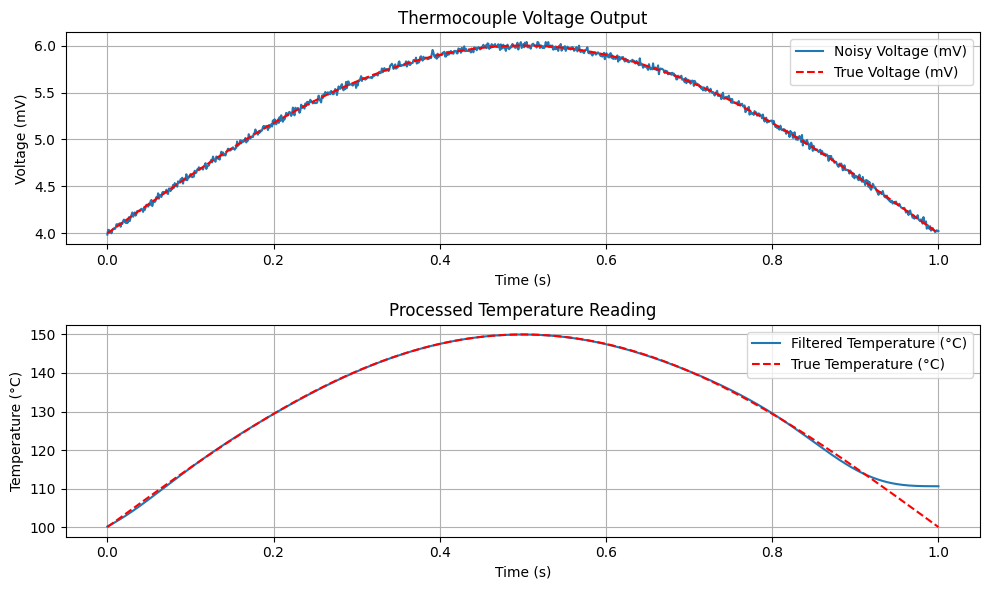
\includegraphics[width=\textwidth]{noisy_signal1.png}
        \caption{Case 1: Low noise, moderate temperature range}
        \label{fig:case1}
    \end{subfigure}
    \begin{subfigure}[b]{0.8\textwidth}
        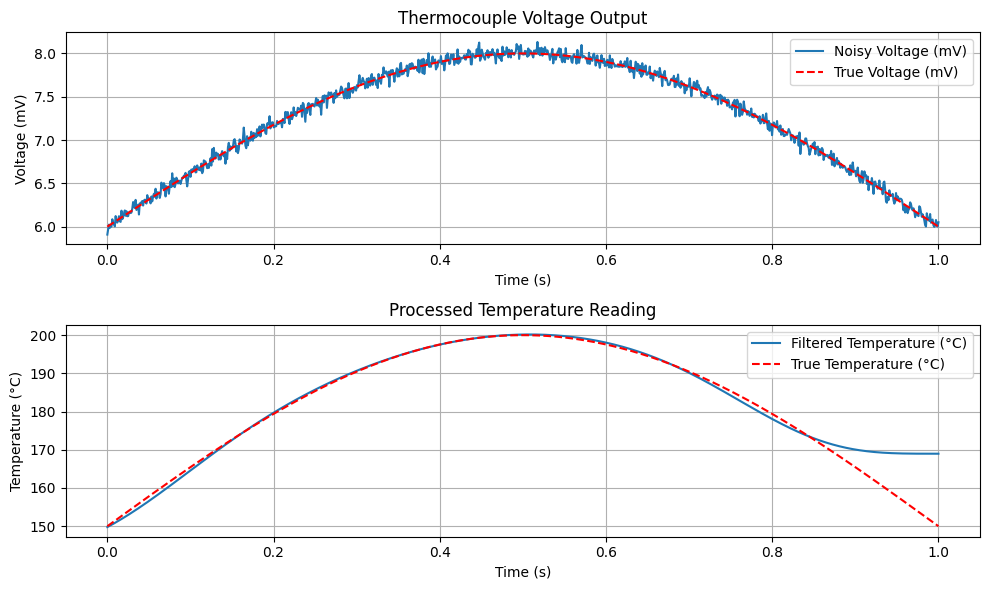
\includegraphics[width=\textwidth]{noisy_signal2.png}
        \caption{Case 2: Medium noise, lower temperature range}
        \label{fig:case2}
    \end{subfigure}
    \begin{subfigure}[b]{0.8\textwidth}
        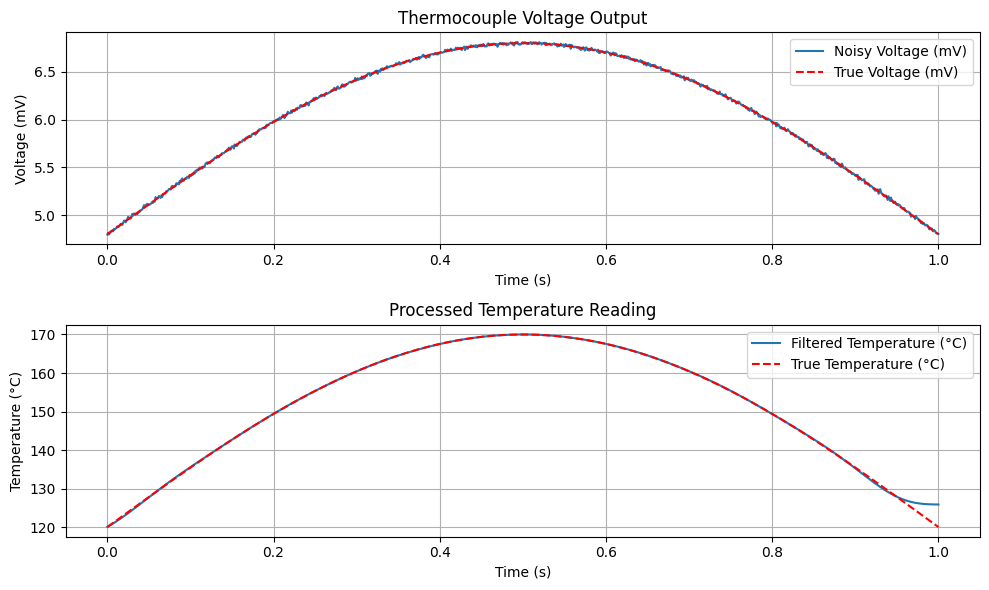
\includegraphics[width=\textwidth]{noisy_signal3.png}
        \caption{Case 3: Higher noise, higher temperature range}
        \label{fig:case3}
    \end{subfigure}
    \caption{Thermocouple Voltage Output and Processed Temperature Reading for Different Cases}
\end{figure}

\section*{Conclusion}
This project successfully simulates a thermocouple-based temperature instrumentation system, demonstrating the integration of sensor modeling, noise simulation, and digital filtering in Python. The theory and mathematical analysis highlight the importance of proper filter design to balance noise reduction with signal preservation. The results from varied parameters show that while the Butterworth filter can smooth noisy signals (as seen in the plots), inappropriate cutoff frequencies or high orders may introduce errors, leading to higher RMSE after filtering in some cases—as observed in Case 3 (RMSE increasing from 1.26°C to 3.95°C with \texttt{cutoff = 3} Hz). Adjusting \texttt{cutoff} to 8 Hz with lower noise (\texttt{noise\_amplitude = 0.01} mV) preserved more signal detail but retained some noise, while the higher temperature range (\texttt{temp\_true = 150 + 50}) with stricter filtering showed over-smoothing. This underscores the need for parameter tuning, such as aligning the cutoff with the signal frequency (0.5 Hz here) and adjusting based on noise levels. Overall, the simulation provides valuable insights into instrumentation challenges and serves as an educational tool for EEE students to explore signal processing without hardware. Future enhancements could include non-linear calibration curves or adaptive filters for better performance.

\end{document}